
\documentclass[10pt,journal,compsoc]{IEEEtran}

\usepackage[pdftex]{graphicx}
\usepackage{caption}

% correct bad hyphenation here
\hyphenation{op-tical net-works semi-conduc-tor}


\begin{document}

\title{EECS 470 Computer Processor Design Report}

\author{Jiale~Huang,~Bryce~Paputa,~Sagar~Sadasivan,~Nathan~Schell,~Yi~Zhi~Wee}% <-this % stops a space

\IEEEtitleabstractindextext{%
\begin{abstract}
Computer processors have changed substantially over the past 50 years in both underlying transistor technology and architecture. Until the early 1990s, consumer processors executed instructions in program order, as one might expect. In order to improve performance, out-of-order execution was introduced to remove unnecessary stalling. For this project, we developed an out-of-order processor based on the MIPS R10k microarchitecture used in the late 1990s, with advanced features such as a superscalar pipeline and early single cycle branch recovery. We also created an advanced memory system to improve performance. This paper outlines the design of our processor and explains the performance improvements from different features. The final clock period for our processor is 13.5ns and we have an average CPI value of 1.35 over the given tests.
\end{abstract}}

% make the title area
\maketitle


\IEEEdisplaynontitleabstractindextext

\IEEEpeerreviewmaketitle

\IEEEraisesectionheading{\section{Project Description}\label{sec:description}}
\IEEEPARstart{T}{he} primary goal of the EECS 470 major design project was to build an out-of-order processor that implements a subset of the Alpha64 ISA (instruction set architecture). Most of our design aspects were taken from the MIPS R10k. The processor is implemented in SystemVerilog hardware description language, and is simulated and synthesized using industry standard tools called Synopsys VCS and Design Compiler respectively. These goals and requirements may seem rather specific, but many design choices were made within a group of technical requirements. The technical requirements are broken up into core features, starred features, optional features, and general requirements. Our complete list of features include:
\begin{itemize}
\item Automated regression testing infrastructure
\item 2-way superscalar
\item Early (pre-retire) recovery from branches
\item Store-to-load forwarding in LSQ
\item Loads issue out-of-order past pending stores
\item Multiple outstanding load misses
\item Stride prefetching for instructions
\item Multi-banked cache
\end{itemize}

\subsection{Core Features}
The most important design requirement for the project is an out-of-order processor. Each group can follow the design methodology of the Intel P6 or MIPS R10k processor for scheduling instructions out of order. Our team chose to follow the R10k implementation as it allows for better performance despite its higher design complexity.

The processor must also use dynamic branch prediction, implemented using a branch target buffer and a bimodal branch predictor (more complex predictions are optional). Instruction execution must be implemented using multiple functional units of varying latencies, and memory accesses must go through the instruction cache or data cache.

% needed in second column of first page if using \IEEEpubid
%\IEEEpubidadjcol

\subsection{Starred Features}
At least one of four “starred” requirements must be implemented. We pursued a 2-way superscalar pipeline to drastically improve performance. Although the 3-way and N-way designs were also available options, complexity increases exponentially with these methods, and performance gains fall off rather quickly. Therefore, we chose the 2-way superscalar pipeline.

Additionally, we chose to implement single cycle pre-retirement branch recovery. This allows us to recover from branch mispredictions quicker; the alternative to this is implementing serial rollback, which takes many cycles to recover the state of the processor. 

\subsection{Optional Features}
Optional features are required to obtain difficulty points and improve our processor’s performance. Our project includes automated regression testing to ensure correctness as more performance features are added. We also added a store queue with store to load forwarding, non-blocking instruction and data cache, dual banked instruction cache, and prefetching. These are important improvements, as the memory system is the slowest part of the processor and a common bottleneck for performance. Also, since we implemented two “starred” features, the early branch recovery is considered optional.

\subsection{General Requirements}
Though it may seem obvious, the most crucial requirement for the project is a correct implementation of the pipeline. It’s easy to get lost in performance improvements, but if the processor doesn’t function perfectly every time, there is little importance in how quickly it runs. Moreover, it is required that each team use some form of revision control with their project to ensure that code is not lost or irreparably modified. Our team used Git paired with a Bitbucket repository for easy viewing and code submission.

\section{Scheduling and Pipeline Design}
Out-of-order processing can be implemented in two ways---copy based renaming and true register renaming. We chose to do true register renaming similar to the MIPS R10k processor. Please refer to appendix A for a high level block diagram of the pipeline.
\subsection{MIPS R10k Out-of-Order Processing}
The R10k implementation uses true register renaming, which involves using a re-order buffer (ROB) and map table to redirect the output of an instruction from one of the 32 architectural registers to one of the 64 physical registers. This allows instructions to execute as soon as their operands are ready; hence reducing the time that the processor must stall compared to an in-order processor.

\subsection{2-Way Superscalar Pipeline}
A superscalar processor can execute multiple instructions in parallel at every point in the pipeline. The main barrier to superscalar performance gain is lack of instruction level parallelism. If a program has many dependencies, increasing the pipeline width has diminishing marginal gains. Furthermore, a wider pipeline introduces additional complexity and implementation effort. For our processor, two instructions can be fetched, dispatched, issued, and completed in a single cycle. We chose a 2-way pipeline over wider ones because of they have higher complexity and diminishing gains, and also because we can only fetch two instructions at a time from memory.

\subsection{Early Single Cycle Branch Recovery}
The simplest way to recover from mispredicted branches involves waiting for the branch to retire and then serially rolling back the state. This takes a long time. Hence, we implemented early single cycle branch recovery. We use a branch resolution stack that keeps track of the recovery state for up to four nested branches, and a branch resolution bus that sends the branch results to the rest of the pipeline a single cycle after the branch is issued to execution. This gives us much better performance than the standard retirement serial roll back method.

\section{Memory System Design}
For this project, the memory system is limited to a single 64-bit data port with 100ns latency. This is a bottle neck for many programs, so we have numerous improvements that attempt to hide the memory latency.

\subsection{Non-blocking and Multi-banked Caches}
To maximize the memory throughput, we implemented non-blocking instruction and data caches. The non-blocking caches allow us to send and receive a memory operation every cycle, regardless of memory latency. Additionally, our instruction cache has two even-odd interleaved banks, allowing us to fetch from from multiple cache blocks when fetching from odd program counters.

\subsection{Prefetching}
Prefetching is introduced to minimize the fetch stage stalling. Our prefetcher sequentially fetches instructions ahead of the actual fetch stage and stores them in the instruction cache. One improvement we made was adapting the prefetch limit distance based on the program code size. Larger programs are more likely to introduce cache conflicts than smaller ones, so fewer instructions should be prefetched. This improvement gave us the benefit of unlimited prefetching on smaller programs, and smaller and more reasonable prefetching distance on larger programs to prevent cache evictions.

\subsection{Store Queue}
We have a store queue which allows loads to execute out of order. Without a store queue, we would not be able to issue loads until there were no in flight stores. The store queue keeps track of which stores the loads could be dependent on and controls their issuing. We also implemented store to load forwarding which allows loads to take data directly from the stores that they are dependent on. Our non-blocking data cache also allows us to have multiple outstanding load misses at a time, improving the performance of sequential loads. We considered, but did not have enough time to add a load queue, which would have allow us to execute loads speculatively. Due to some implementation details of our non-blocking cache and CDB arbitration, without a load queue we can only issue a single load in a cycle.
\section{Pipeline Details}
All of the modules that we created work correctly and synthesize without latches or timing loops.
\begin{itemize}
\item The fetch stage fetches two instructions each cycle, and will fetch from predicted branches.
\item The branch target buffer and branch history table are both direct mapped caches with 256 entries each.
\item There is a circular instruction buffer between the fetch and dispatch stages with eight entries.
\item The re-order buffer is a circular buffer with 32 entries.
\item The reservation station is fully associative, i.e. any entry can be dispatched to at any time regardless of functional unit type.
\item The map table is a map of 32 architectural registers to 64 physical registers, with ready bits.
\item The free list is a circular buffer of up to 32 available tags.
\item The branch stack has four entries that keep track of free list, re-order buffer and store queue tails, and also and the map table contents
\item There are two ALUs, two four-stage multipliers, one branch module, and one memory module (that can take two instructions per cycle).
\item Each functional unit has a two-entry output buffer that the common data bus gets the results from.
\item The common data bus can complete two instructions per cycle.
\item The memory datapath contains an eight-entry store queue, a non-blocking and two-banked-interleaved instruction cache, and a non-blocking data cache.
\item The non-blocking caches share a 15-entry miss status handle register table.
\item The instruction cache has two banks of 16 eight-byte wide lines. The data cache has 32 eight-byte wide lines.
\item The branch functional unit broadcasts branch results to the entire processor for a single cycle after they are computed.
\end{itemize}
\section{Verification and Testing}
We used a few different techniques to verify that our processor is correct: unit testing, regression testing, and using testbench outputs.
\subsection{Unit Testing}
Unit testing separates a section of code from the rest of the system and verifies that it performs as expected given all, or nearly all, possible inputs (especially corner cases and stress tests). Unit testing played a particularly large part in verification early in the development process. Integration testing using full test programs was impossible before the pipeline was fully implemented, so unit tests were created for most modules to ensure the correctness of each module and reduce debugging time during pipeline integration. Some sections of code were either so small and simple as to not warrant unit testing, or were provided in the original course code (e.g. the decoder). Once the pipeline was fully completed, debugging using actual test programs proved much more useful in exposing and identifying bugs, as many of the bugs in our pipeline were caused by faulty integration of different modules, and these bugs would not appear in the unit tests.

\subsection{Automated Regression Testing}
There were a variety of automated testing scripts that were used throughout the development process. Early on, we used a bash script that simply built each of the modules and ran their respective unit tests. This was useful to ensure that modules weren’t broken accidentally, and to provide direction about which modules needed work most urgently. Once we could start running our processor against assembly code test cases, a bash script was written to build the baseline processor from project 3 and run our test programs. The script then built our current processor and ran the same test programs it, and verified that the final register and memory states matched. This provides a simple passed/failed output on each case, and highlighted what registers or memory locations differed in the case of a failure. Lastly, once we were getting close to being done we made a script that ran every test program, recorded, and graphed stats such as CPI and total execution time. From there, we were able to deduce which tests were the slowest, and decide on what modules to improve.

\subsection{Testbench Outputs}
Alongside the automated script for integration testing, the most important debugging tool for the fully implemented processor was once per cycle debugging outputs from the testbench. Each module’s debugging outputs were printed from their own Verilog task in the testbench, so the outputs for certain modules could be easily enabled and disabled by commenting out the function calls in the main loop. The outputs were much cleaner and more understandable than other tools like DVE, and outputting in the testbench at a clock edge provides more predictable timing than outputs placed in the modules themselves. 

\section{Team Division of Work}
We worked together as a group for the first few modules (RS and ROB). After that, we worked as follows:
\begin{description}
\item [Jiale] Instruction buffer, SQ, CDB
\item [Bryce] Cache controllers, SQ, MT, FL, branch FU, IF, Prefetch, branch stack
\item [Sagar] Synthesis, MT, FL, FU buffer
\item [Nathan] Cache controllers, FU buffer, CDB, registers, Prefetch
\item [Yi Zhi] Branch prediction, FU buffer, mult FU, IF, branch stack

\end{description}
We all put in approximately equal amounts of work in terms of time, and all worked on testing of our own modules and their integration to others.

\section{Performance Analysis}
There are two primary measures of performance for our processors. The first is the clock period (the time required for a single cycle), which is determined by the results of synthesis. A lower clock period is better, but more complex modules that provide other benefits will increase the clock period substantially. This must be balanced with the cycles per instruction (CPI, the number of clock cycles required to finish one instruction), which should be as low as possible. CPI is different for each program that the processor runs, but comparisons can be made between processors by running the same programs. Ultimately, the CPI and clock period are used to calculate the overall throughput of the processor, in instructions per second (calculated by taking the reciprocal of CPI multiplied by the clock period). This is a consistent metric for comparing processors to one another, assuming the CPI is calculated using the same test programs. Table 1 below summarizes the performance of our final pipeline with the given tests; it has a 13.5ns clock period and 1.35 average CPI.

If pipelines have the same clock period, only the CPI is required for performance analysis. Since it takes a significant amount of time to determine clock period via synthesis, we only compared CPI between feature sets. Therefore, with the assumption that all our different feature sets have the same clock period, the superscalar, non-blocking caches, and fast branch recovery, would have slightly exaggerated performance improvements.

\begin{table}[!htb]
\centering
\begin{tabular}{l | r | r | r}
	Test Program & Size & CPI & Total Time ($\mu s$) \\
	\hline
	objsort & 19704 & 1.654 & 440.08\\
	fib\textunderscore rec & 12942 & 1.397 & 244.06 \\
	parsort & 11106 & 1.079 & 161.82 \\
	sort & 1349 & 1.302 & 23.71\\
	fib\textunderscore long & 627 & 0.536 & 4.52 \\
	insertion & 598 & 0.923 & 7.43\\
	copy\textunderscore long & 590 & 0.537 & 4.26\\
	btest2 & 455 & 3.158 & 19.39\\
	mult & 325 & 1.489 & 6.52 \\
	evens\textunderscore long & 318 & 0.714 & 3.05\\
	btest1 & 229 & 3.611 & 11.15\\ 
	parallel & 194 & 0.675 & 1.76\\
	fib & 147 & 0.850 & 1.67\\
	copy & 130 & 0.908 & 1.58\\
	evens & 82 & 1.402 & 1.54	
\end{tabular}
\caption{Performance on the given test programs}
\end{table}

\begin{figure*}[!htb]
\centering
\captionsetup{justification=centering}
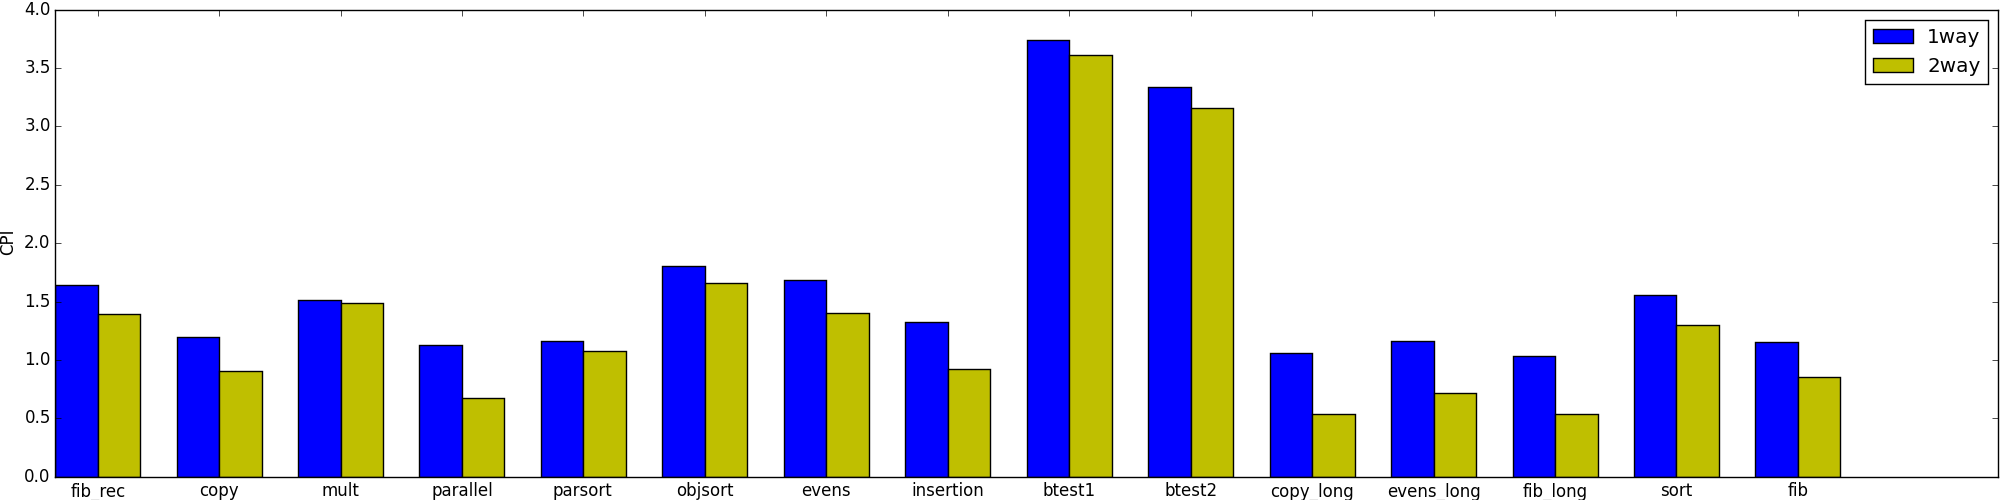
\includegraphics[width=\textwidth]{superscalar}
\caption{Graph of superscalar performance compared to scalar performance\newline}
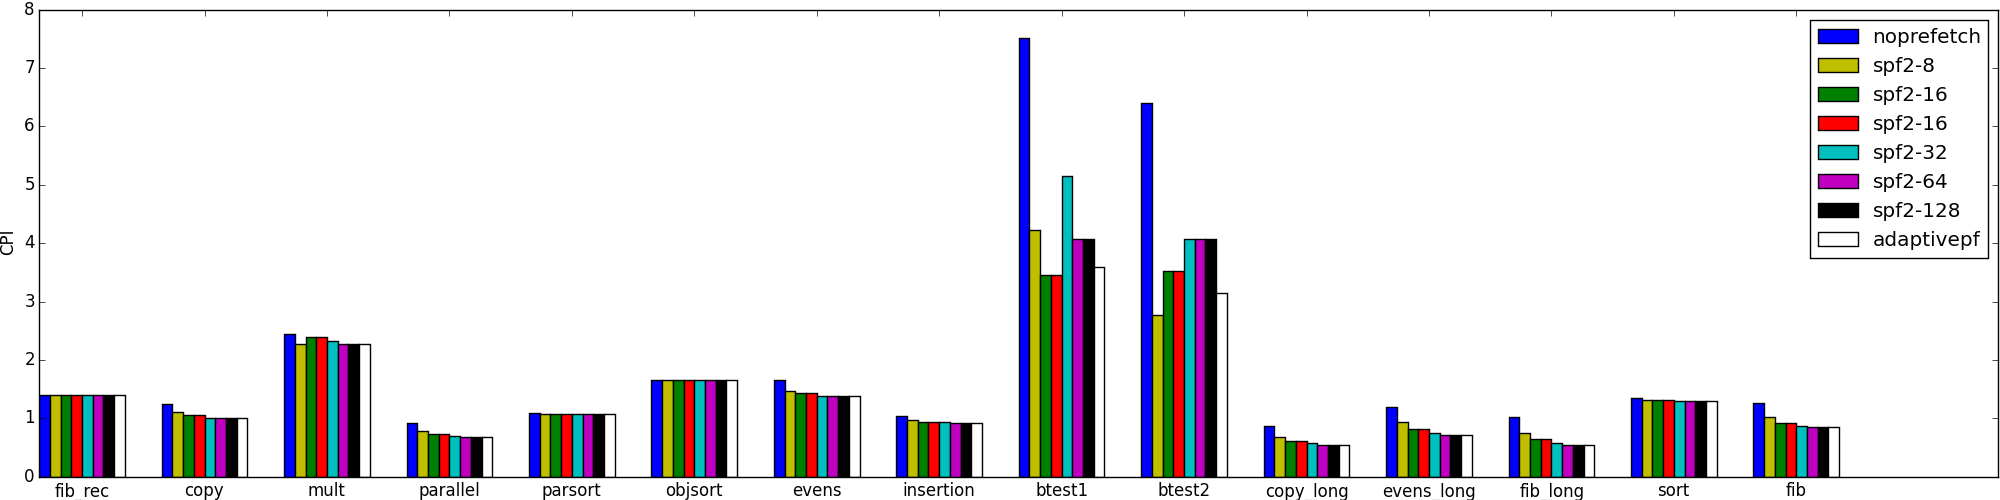
\includegraphics[width=\textwidth]{prefetching}
\caption{Graph of different prefetcher performances}
\end{figure*}
\newpage

\subsection{Superscalar Analysis}
Going from scalar to 2-way superscalar gave us an average 22\% CPI improvement, and improved every single test case. This is shown above in figure 1. We expected this, as it was our main pipeline improvement. The best improvement gains come from highly parallel programs like ``parallel'' and the ``long'' tests. ``mult'' gets little improvement as it consists of many long dependent multiplications. ``btest'' suffers from many branch mispredictions, so it also gets little improvement.

\subsection{Prefetching Analysis}

Prefetching (along with the prerequisite non-blocking instruction cache) gives a substantial average CPI improvement of 23\%. Our simple prefetcher (labeled spf2-X in the graph) sequentially fetches instructions up to X bytes ahead of the fetch stage. While prefetching improves performance by reducing memory wait time, prefetching too far ahead can cause cache conflicts and reduce performance. This section aims to find the most optimized prefetcher for our project. The results are demonstrated in figure 2 above, and table 2 in the next page.

We tried two improvements on the simple prefetcher, the first one uses the BTB to fetch from predicted branches. This performed worse than the simple prefetcher on moderate settings. The first time we encounter a branch instruction, we do not calculate its target address until execution, which is too late for the prefetcher to use. A fix for this would involve speculatively calculating branch target addresses in the fetch stage when they are dispatched, and using the results to prefetch and help with branch predictions before the BTB entry was generated. We did not have time to implement and evaluate this option, so the predicting prefetcher never performed well.

The second improvement adapts the prefetching limit distance based on program size. Programs with basic blocks that are large compared to the total program size are less likely to have cache conflicts caused by aggressive prefetching. If the basic blocks are relatively small, or significantly spread out, aggressive prefetching will often evict useful instruction data. For example, the btest programs, which consist entirely of small 16 byte blocks, show the best performance with prefetching limited to 8-16 bytes. On the other hand, programs like the ``long'' programs, which consist of a single larger basic block, show performance continuous performance improvements with increased prefetching limits. Calculating the exact basic block size is hard to do in time to use it for prefetching (see the problems with the first improvement), but program code size is easy to estimate once the program starts running. We track the largest program counter that the processor has encountered and reduce the prefetching distance when it gets to certain sizes. This allows us to pick a very good limit for each program and get a 23\% improvement over no prefetcher, significantly helping our worst case programs. 

\begin{table}[!htb]
\centering
\begin{tabular}{l | c}
	Prefetcher & CPI Improvement (\%) \\
	\hline
	8 & 16.4 \\
	16 & 19.2\\
	32 & 19.5 \\
	64 & 21.8 \\
	128 & 21.8 \\
	adaptive & 23.1
\end{tabular}
\caption{List of average prefetcher performance}
\end{table}

\begin{figure*}
\centering
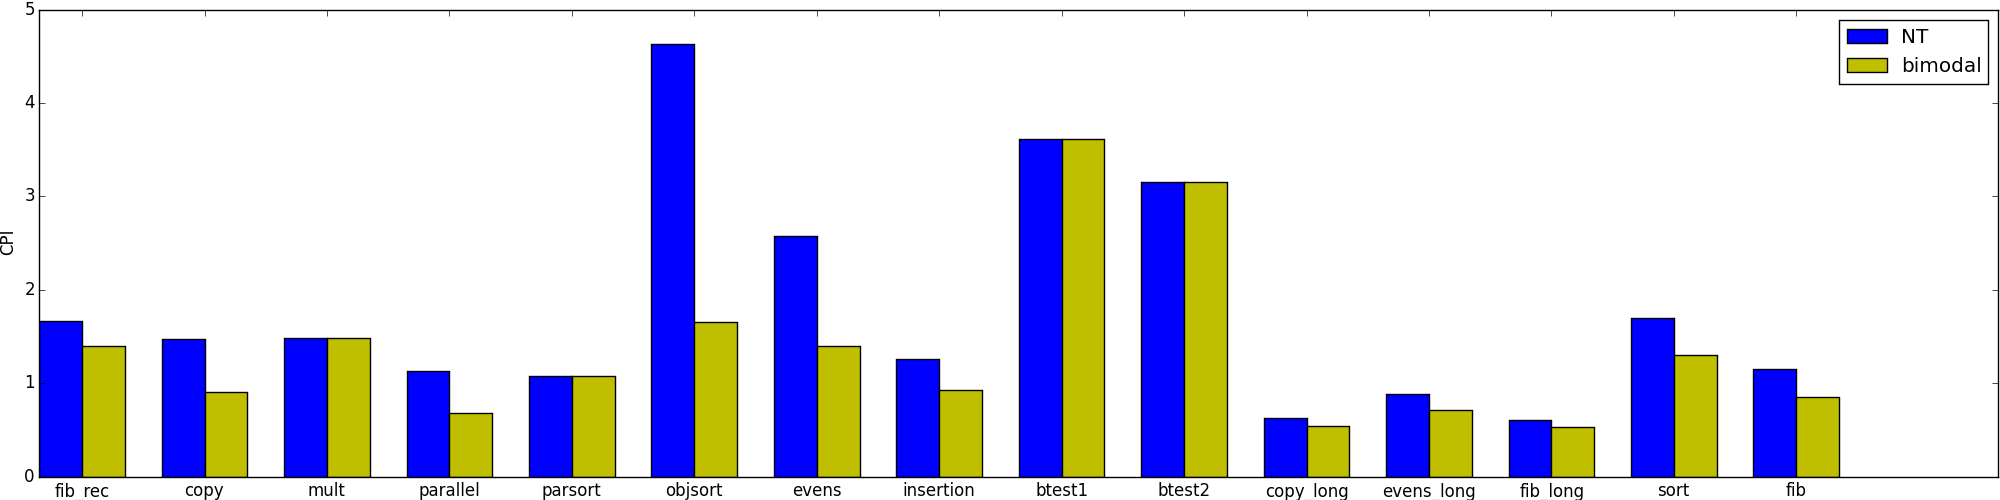
\includegraphics[width=\textwidth]{branchprediction}
\caption{Branch prediction performance improvement}
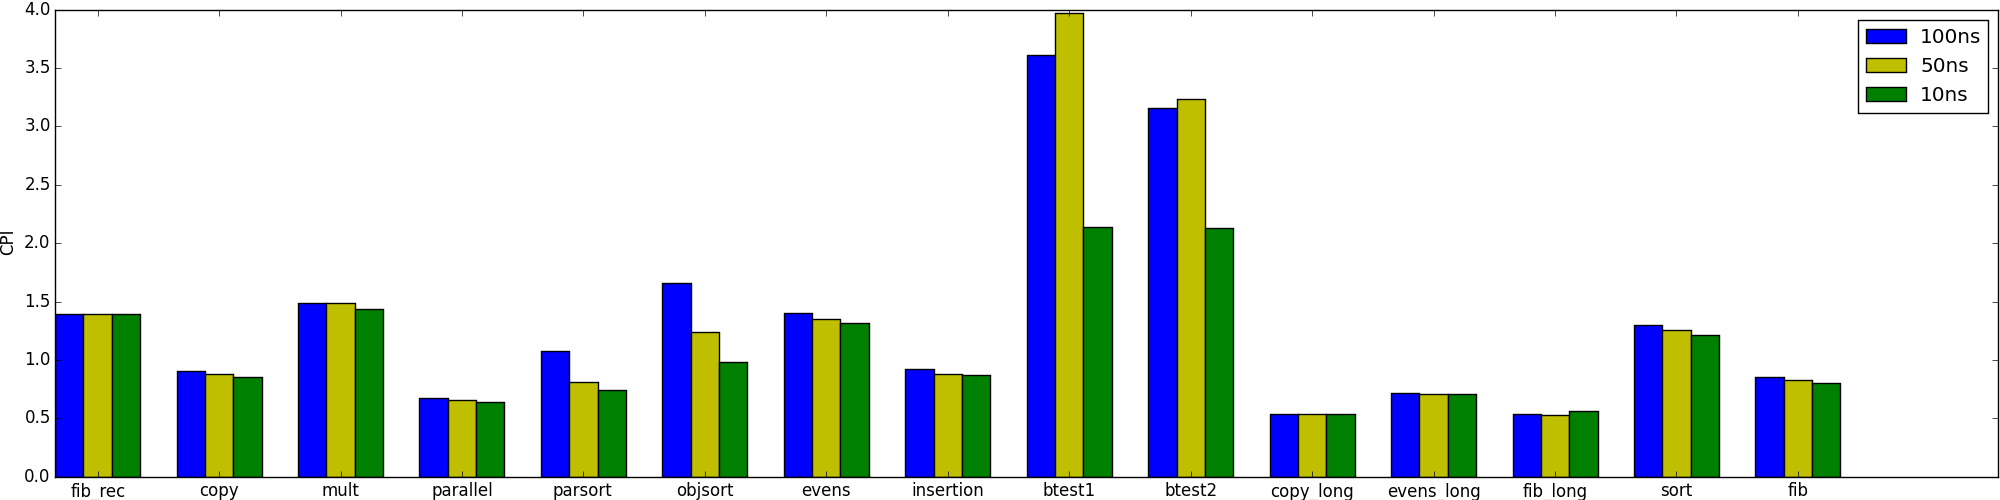
\includegraphics[width=\textwidth]{memlatency}
\caption{Performance under differing memory latencies}
\end{figure*}

\subsection{Branch Prediction Analysis}
The bimodal branch predictor allows the processor to predict which control paths will be taken and speculatively execute them. It keeps a branch history table that has a two bit saturating counter that tracks direction history for every branch, and uses a branch target buffer to cache branch target addresses. This gives us a 91\% prediction accuracy. We considered implementing more advanced branch predictors like tournament predictors and using global history buffers, but we were advised not to. The test programs and workloads given for this project are relatively small and do not see much improvement from deeper or more complex history tracking.

Figure 3 above shows our performance improvements from always predicting not taken to using our branch predictor. Table 3, on the right, shows our branch prediction accuracy for each test program. Many of the programs have very few branches because they are generally small programs. This gives them a disproportionately high miss rate because it takes relatively longer to warm up the BTB and BHT. This led us to choose to not implement more advanced branch predictors.

The btest programs are extreme outliers when looking at accuracy. This is because there are many branches and each branch is only visited once. We are never able to predict taken at any of the branches because the target addresses are not in the BTB yet, so we are only correct on the not taken branches. We could potential improve this with a global predictor and early target address calculation.

\begin{table}[!htb]
\centering
\begin{tabular}{l | r | r}
	Test Program & \# Branches & Accuracy (\%) \\ 
	\hline
	objsort & 8302 & 98.4 \\
	fib\textunderscore rec & 5478 & 84.5 \\
	parsort & 561 & 93.2 \\
	sort & 302 & 64.6 \\
	btest2 & 192 & 33.3 \\
	insertion & 164 & 87.2 \\
	btest1 & 96 & 33.3 \\
	evens & 33 & 69.7 \\
	evens\textunderscore long & 32 & 68.8 \\
	mult & 17 & 82.4 \\
	copy & 16 & 87.5 \\
	parallel & 16 & 87.5 \\
	copy\textunderscore long & 16 & 87.5 \\
	fib\textunderscore long & 14 & 85.7 \\
	fib & 14 & 85.7 \\
	\hline
	\textbf{Total:} & & \textbf{91.0}
\end{tabular}
\caption{Branch prediction accuracy}
\end{table}
\newpage

\subsection{Memory Latency}
Looking at performance while varying memory latency can show how effective we are at hiding the memory latency. Figure 4 above illustrates our pipeline's performance under differenct latencies. Our ability to hide the latency varies dramatically between programs. ``objsort'' shows the most improvement with lower memory latencies because it uses memory a lot. The \textunderscore long programs show almost no difference with between different latencies; this is because we are able to hide the latency well enough that something else becomes the limiting factor. Other programs have similar results too. Interestingly, the ``btest'' programs perform better at 100ns than 50ns, likely because they are highly dependent on prefetcher tuning. If we tuned our prefetcher aggression curve at 50ns, it should perform better.

\appendices
\section{High Level Block Diagram}
\begin{figure}[!htb]
\centering
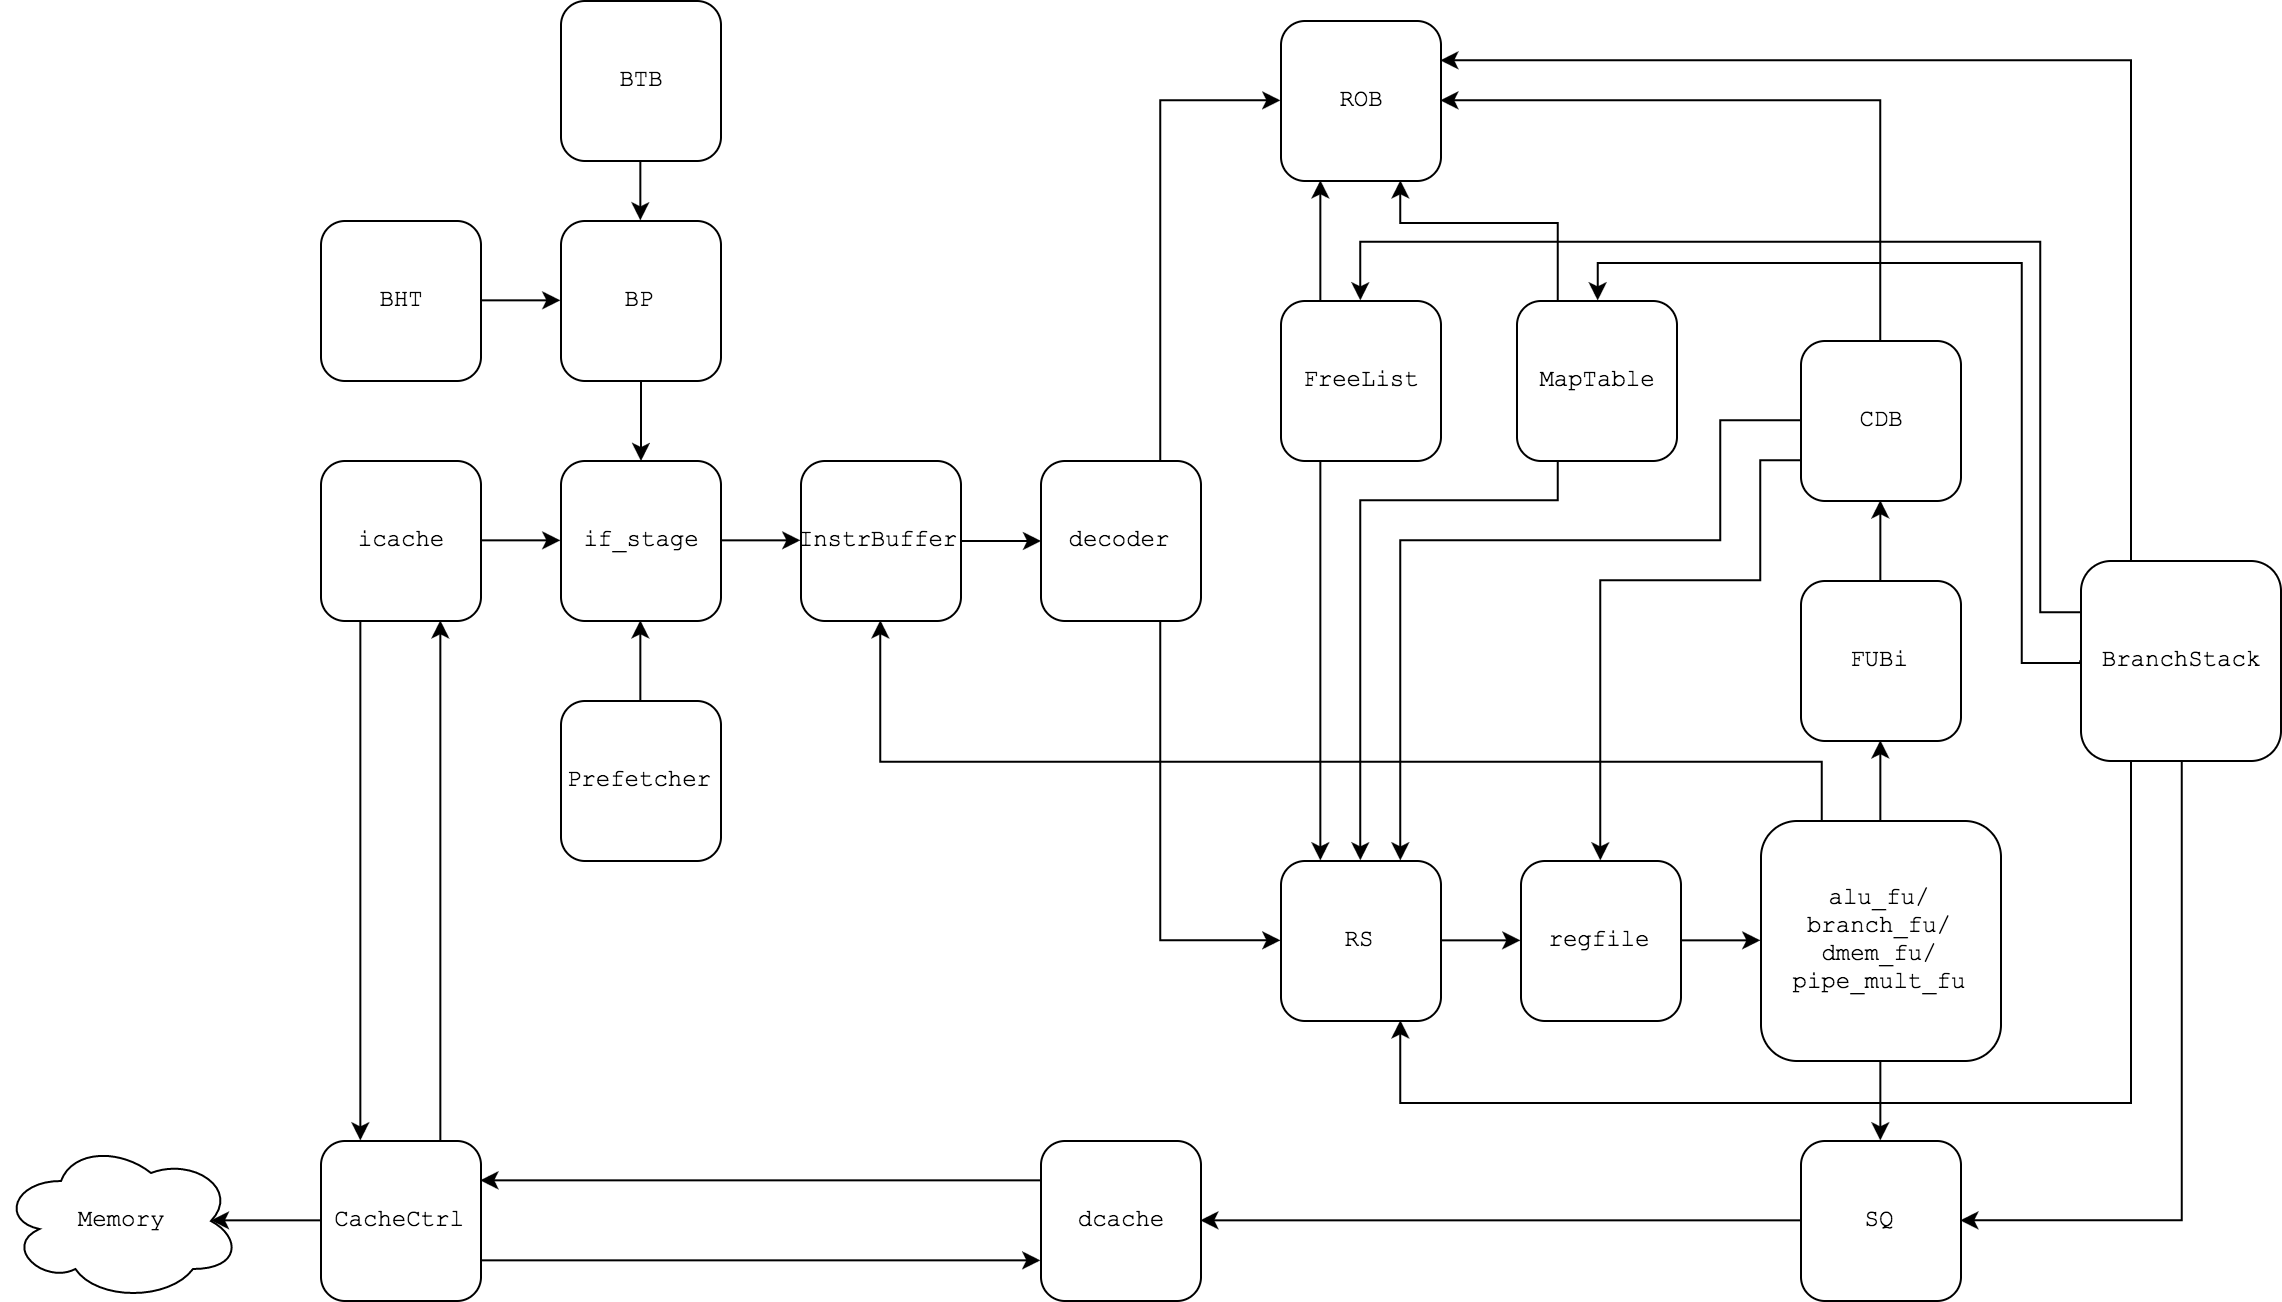
\includegraphics[width=\textwidth]{blocks}
\end{figure}

% that's all folks
\end{document}


